% Options for packages loaded elsewhere
\PassOptionsToPackage{unicode}{hyperref}
\PassOptionsToPackage{hyphens}{url}
\PassOptionsToPackage{dvipsnames,svgnames,x11names}{xcolor}
%
\documentclass[
  12pt,
]{article}
\usepackage{amsmath,amssymb}
\usepackage{lmodern}
\usepackage{setspace}
\usepackage{iftex}
\ifPDFTeX
  \usepackage[T1]{fontenc}
  \usepackage[utf8]{inputenc}
  \usepackage{textcomp} % provide euro and other symbols
\else % if luatex or xetex
  \usepackage{unicode-math}
  \defaultfontfeatures{Scale=MatchLowercase}
  \defaultfontfeatures[\rmfamily]{Ligatures=TeX,Scale=1}
  \setmainfont[]{Arial}
\fi
% Use upquote if available, for straight quotes in verbatim environments
\IfFileExists{upquote.sty}{\usepackage{upquote}}{}
\IfFileExists{microtype.sty}{% use microtype if available
  \usepackage[]{microtype}
  \UseMicrotypeSet[protrusion]{basicmath} % disable protrusion for tt fonts
}{}
\makeatletter
\@ifundefined{KOMAClassName}{% if non-KOMA class
  \IfFileExists{parskip.sty}{%
    \usepackage{parskip}
  }{% else
    \setlength{\parindent}{0pt}
    \setlength{\parskip}{6pt plus 2pt minus 1pt}}
}{% if KOMA class
  \KOMAoptions{parskip=half}}
\makeatother
\usepackage{xcolor}
\usepackage[margin=1in]{geometry}
\usepackage{longtable,booktabs,array}
\usepackage{calc} % for calculating minipage widths
% Correct order of tables after \paragraph or \subparagraph
\usepackage{etoolbox}
\makeatletter
\patchcmd\longtable{\par}{\if@noskipsec\mbox{}\fi\par}{}{}
\makeatother
% Allow footnotes in longtable head/foot
\IfFileExists{footnotehyper.sty}{\usepackage{footnotehyper}}{\usepackage{footnote}}
\makesavenoteenv{longtable}
\usepackage{graphicx}
\makeatletter
\def\maxwidth{\ifdim\Gin@nat@width>\linewidth\linewidth\else\Gin@nat@width\fi}
\def\maxheight{\ifdim\Gin@nat@height>\textheight\textheight\else\Gin@nat@height\fi}
\makeatother
% Scale images if necessary, so that they will not overflow the page
% margins by default, and it is still possible to overwrite the defaults
% using explicit options in \includegraphics[width, height, ...]{}
\setkeys{Gin}{width=\maxwidth,height=\maxheight,keepaspectratio}
% Set default figure placement to htbp
\makeatletter
\def\fps@figure{htbp}
\makeatother
\setlength{\emergencystretch}{3em} % prevent overfull lines
\providecommand{\tightlist}{%
  \setlength{\itemsep}{0pt}\setlength{\parskip}{0pt}}
\setcounter{secnumdepth}{5}
\newlength{\cslhangindent}
\setlength{\cslhangindent}{1.5em}
\newlength{\csllabelwidth}
\setlength{\csllabelwidth}{3em}
\newlength{\cslentryspacingunit} % times entry-spacing
\setlength{\cslentryspacingunit}{\parskip}
\newenvironment{CSLReferences}[2] % #1 hanging-ident, #2 entry spacing
 {% don't indent paragraphs
  \setlength{\parindent}{0pt}
  % turn on hanging indent if param 1 is 1
  \ifodd #1
  \let\oldpar\par
  \def\par{\hangindent=\cslhangindent\oldpar}
  \fi
  % set entry spacing
  \setlength{\parskip}{#2\cslentryspacingunit}
 }%
 {}
\usepackage{calc}
\newcommand{\CSLBlock}[1]{#1\hfill\break}
\newcommand{\CSLLeftMargin}[1]{\parbox[t]{\csllabelwidth}{#1}}
\newcommand{\CSLRightInline}[1]{\parbox[t]{\linewidth - \csllabelwidth}{#1}\break}
\newcommand{\CSLIndent}[1]{\hspace{\cslhangindent}#1}
\usepackage[left]{lineno}
\linenumbers
\usepackage{subfig}
\ifLuaTeX
  \usepackage{selnolig}  % disable illegal ligatures
\fi
\IfFileExists{bookmark.sty}{\usepackage{bookmark}}{\usepackage{hyperref}}
\IfFileExists{xurl.sty}{\usepackage{xurl}}{} % add URL line breaks if available
\urlstyle{same} % disable monospaced font for URLs
\hypersetup{
  pdftitle={My awesome title},
  pdfauthor={Olalla Díaz-Yáñez,},
  colorlinks=true,
  linkcolor={blue},
  filecolor={Maroon},
  citecolor={Blue},
  urlcolor={Blue},
  pdfcreator={LaTeX via pandoc}}

\title{My awesome title}
\author{Olalla Díaz-Yáñez,}
\date{2023-04-11}

\begin{document}
\maketitle

\setstretch{1.5}
\hypertarget{abstract}{%
\section{Abstract}\label{abstract}}

Lorem ipsum dolor sit amet. At perspiciatis iusto est assumenda alias et distinctio voluptas non perspiciatis eveniet! Est similique nisi id debitis ipsa cum libero quibusdam eos quia esse cum esse fugiat sit cupiditate impedit. Aut architecto velit qui voluptatem similique vel placeat expedita et incidunt reiciendis et quos tempore. 33 voluptatibus voluptatem et magni aspernatur sed aspernatur dolorem ut aspernatur blanditiis.

Et expedita impedit aut voluptatum quia ut perspiciatis earum. Eum voluptatum cumque ut rerum quam et illum exercitationem sit accusantium dolorum et modi reprehenderit ut velit voluptatem.

At quia omnis sit laudantium sunt non aperiam cupiditate et nobis magni et voluptatem perspiciatis. Eum natus harum quo rerum esse hic eveniet omnis aut blanditiis internos aut tempora obcaecati sed molestiae illum.
\newpage

\hypertarget{introduction}{%
\section{Introduction}\label{introduction}}

Here I add a reference (\protect\hyperlink{ref-foresteurope2020}{FOREST EUROPE, 2020}).
Here I add two references (\protect\hyperlink{ref-bugmann1996}{Bugmann et al., 1996}; \protect\hyperlink{ref-vanclay1997}{Vanclay \& Skovsgaard, 1997}),
and I add another sentence with more references (\protect\hyperlink{ref-bugmann2019}{Bugmann et al., 2019}; \protect\hyperlink{ref-cailleret2017}{Cailleret et al., 2017}). 2; Lexer \& Hönninger (\protect\hyperlink{ref-lexer2001}{2001}); Reyer et al. (\protect\hyperlink{ref-reyer2014}{2014}){]}.

\hypertarget{material-and-methods}{%
\section{Material and methods}\label{material-and-methods}}

\hypertarget{subsection}{%
\subsection{Subsection}\label{subsection}}

Lorem ipsum dolor sit amet. At perspiciatis iusto est assumenda alias et distinctio voluptas non perspiciatis eveniet! Est similique nisi id debitis ipsa cum libero quibusdam eos quia esse cum esse fugiat sit cupiditate impedit. Aut architecto velit qui voluptatem similique vel placeat expedita et incidunt reiciendis et quos tempore. 33 voluptatibus voluptatem et magni aspernatur sed aspernatur dolorem ut aspernatur blanditiis.

Et expedita impedit aut voluptatum quia ut perspiciatis earum. Eum voluptatum cumque ut rerum quam et illum exercitationem sit accusantium dolorum et modi reprehenderit ut velit voluptatem.

At quia omnis sit laudantium sunt non aperiam cupiditate et nobis magni et voluptatem perspiciatis. Eum natus harum quo rerum esse hic eveniet omnis aut blanditiis internos aut tempora obcaecati sed molestiae illum.

\hypertarget{results}{%
\section{Results}\label{results}}

Here one example referencing one figure (Figure \ref{fig:ventana}).

\begin{figure}
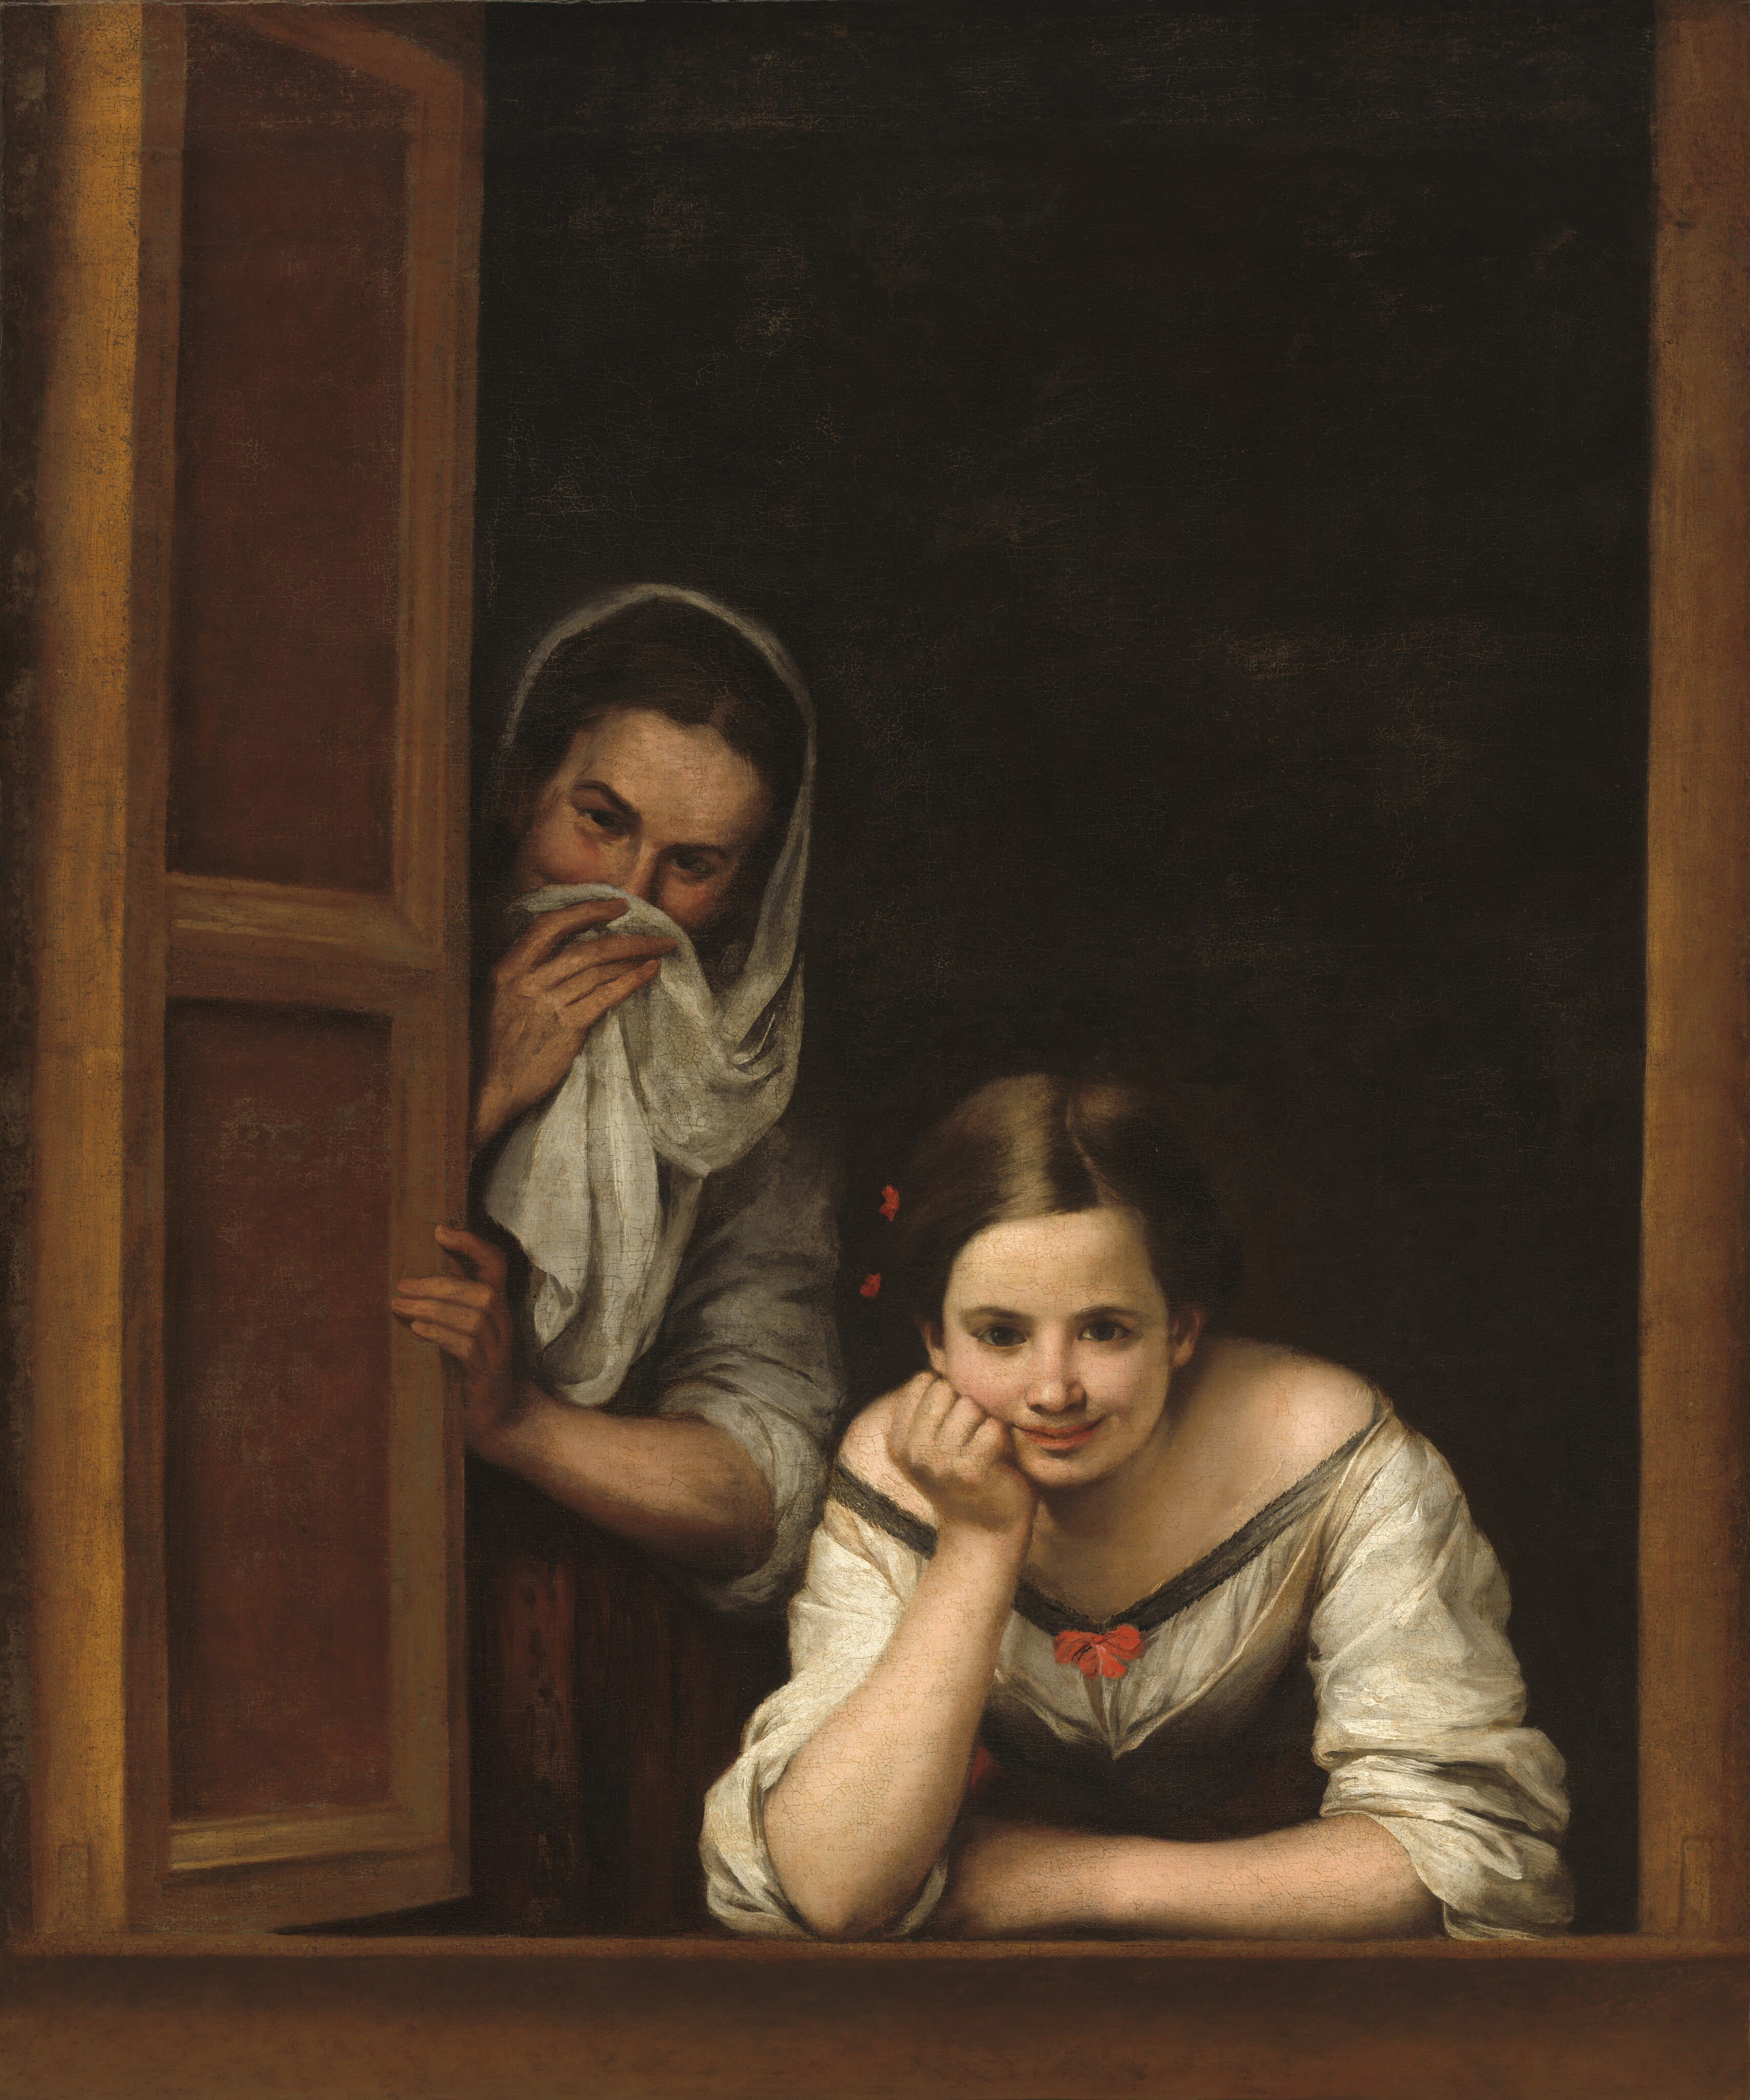
\includegraphics[width=1\linewidth]{../../figures/two_women_at_a_window_1942.9.46} \caption{One example figure with caption}\label{fig:ventana}
\end{figure}

\hypertarget{discussion}{%
\section{Discussion}\label{discussion}}

\hypertarget{references}{%
\section{References}\label{references}}

\hypertarget{refs}{}
\begin{CSLReferences}{1}{0}
\leavevmode\vadjust pre{\hypertarget{ref-bugmann1996a}{}}%
Bugmann, H. (1996). A Simplified Forest Model to Study Species Composition Along Climate Gradients. \emph{Ecology}, \emph{77}(7), 2055--2074. \url{https://doi.org/10.2307/2265700}

\leavevmode\vadjust pre{\hypertarget{ref-bugmann2019}{}}%
Bugmann, H., Seidl, R., Hartig, F., Bohn, F., Brůna, J., Cailleret, M., François, L., Heinke, J., Henrot, A.-J., Hickler, T., Hülsmann, L., Huth, A., Jacquemin, I., Kollas, C., Lasch-Born, P., Lexer, M. J., Merganič, J., Merganičová, K., Mette, T., \ldots{} Reyer, C. P. O. (2019). Tree mortality submodels drive simulated long-term forest dynamics: assessing 15 models from the stand to global scale. \emph{Ecosphere}, \emph{10}(2), e02616. \url{https://doi.org/10.1002/ecs2.2616}

\leavevmode\vadjust pre{\hypertarget{ref-bugmann1996}{}}%
Bugmann, H., Yan, X., Sykes, MartinT., Martin, P., Lindner, M., Desanker, PaulV., \& Cumming, SteveG. (1996). A comparison of forest gap models: Model structure and behaviour. \emph{Climatic Change}, \emph{34}(2). \url{https://doi.org/10.1007/BF00224640}

\leavevmode\vadjust pre{\hypertarget{ref-cailleret2017}{}}%
Cailleret, M., Jansen, S., Robert, E. M. R., Desoto, L., Aakala, T., Antos, J. A., Beikircher, B., Bigler, C., Bugmann, H., Caccianiga, M., Čada, V., Camarero, J. J., Cherubini, P., Cochard, H., Coyea, M. R., Čufar, K., Das, A. J., Davi, H., Delzon, S., \ldots{} Martínez-Vilalta, J. (2017). A synthesis of radial growth patterns preceding tree mortality. \emph{Global Change Biology}, \emph{23}(4), 1675--1690. \url{https://doi.org/10.1111/gcb.13535}

\leavevmode\vadjust pre{\hypertarget{ref-foresteurope2020}{}}%
FOREST EUROPE. (2020). \emph{State of europe{'}s forests 2020.}

\leavevmode\vadjust pre{\hypertarget{ref-lexer2001}{}}%
Lexer, M. J., \& Hönninger, K. (2001). A modified 3D-patch model for spatially explicit simulation of vegetation composition in heterogeneous landscapes. \emph{Forest Ecology and Management}, 23.

\leavevmode\vadjust pre{\hypertarget{ref-reyer2014}{}}%
Reyer, C., Lasch-Born, P., Suckow, F., Gutsch, M., Murawski, A., \& Pilz, T. (2014). \emph{Projections of regional changes in forest net primary productivity for different tree species in Europe driven by climate change and carbon dioxide}.

\leavevmode\vadjust pre{\hypertarget{ref-vanclay1997}{}}%
Vanclay, J. K., \& Skovsgaard, J. P. (1997). Evaluating forest growth models. \emph{Ecological Modelling}, \emph{98}(1), 1--12. \url{https://doi.org/10.1016/S0304-3800(96)01932-1}

\end{CSLReferences}

\end{document}
